\chapter{Αισθητήρες}

\section{Οπτικοί κωδικοποιητές}

Σύμφωνα με έκδοσης της \textcite[12]{drc76}, οπτικοί κωδικοποιητές περιστροφικής
κίνησης, παραδοσιακά, κατασκευάζονται με την προσάρτηση ενός περιφερειακά
διάτρητου δίσκου στον άξονα κίνησης εκατέρωθεν του οποίου διατάσσεται αντικριστό
ζεύγος πομπού και δέκτη υπέρυθρων ακτίνων. Καθώς ο δίσκος περιστρέφεται ως
αποτέλεσμα κίνησης του άξονα, η ύπαρξη ή έλλειψη οπής επαναφέρει ή αποκόπτει την
επικοινωνία μεταξύ πομπού-δέκτη προκαλώντας εναλλαγές στην έξοδο του δέκτη
\parencite[12]{drc76}.

Στην απλούστερη υλοποίηση, ο αισθητήρας αναγνωρίζει τη μετάβαση από τη μία θέση
στην επόμενη ενώ είναι αδύνατο να αναχθεί από το σήμα και μόνον, είτε η φορά
περιστροφής είτε η τρέχουσα γωνιακή μετατόπιση του άξονα· ο ελεγκτής είναι
υπεύθυνος για την εξαγωγή αυτών των συμπερασμάτων \parencites[5--6]{lynch02}
[13]{drc76}. Στην περίπτωση αυτή, ο κωδικοποιητής αποκαλείται
\emph{προσαυξητικός}\index{προσαυξητικός κωδικοποιητής} (\emph{incremental})
\parencite[5]{lynch02}.

Ωστόσο, είναι δυνατό να κατασκευαστεί \emph{απόλυτος} (\emph{absolute})
κωδικωποιητής\index{κωδικοποιητής απόλυτης μετατόπισης} μετατόπισης, κάνοντας
χρήση πολλαπλών ζευγών πομπού-δέκτη και ενός δίσκου υποδιαιρεμένου σε διακριτές
θέσεις που αποτελούνται από μοναδικό συνδυασμό οπών \parencites[6]{lynch02}. Ο
κάθε αισθητήρας παράγει έξοδο ανεξάρτητη από τους υπολοίπους βάσει των οπών που
του αντιστοιχούν, ενώ η συνδυαστική έξοδος όλων των αισθητήρων περιγράφει τον
τρέχοντα συνδυασμό οπών και συνεπώς τη γωνιακή μετατόπιση του δίσκου
\parencites[6]{lynch02}.

Για τη σύνθεση ενός κωδικοποιητή που κάνει χρήση οπτικών αισθητήρων,
χρησιμοποιούνται ζεύγη πομπού και δέκτη υπέρυθρων ακτίνων. Το κάθε ζεύγος μπορεί
να αποτελείται από ανεξάρτητα, μεταξύ τους, στοιχεία ή να βρίσκονται
ενσωματωμένα σε ειδική θήκη που διευκολύνει την τοποθέτησή τους.

Υπάρχουν διατάξεις που τοποθετούν αντικριστά το ζεύγος πομπού και δέκτη
σχηματίζοντας έναν κενό χώρο μεταξύ τους στον οποίο μπορεί να εισέρχεται
εξωτερικό αντικείμενο, διακόπτοντας την επικοινωνία τους. Τέτοιοι αισθητήρες
αναφέρονται ως \emph{φωτοδιακόπτες}\index{φωτοδιακόπτης}
(\emph{photointerrupter}) \parencite[3]{lynch02} και αποτελούν τη διάταξη που
έχει παρουσιαστεί στα μέχρι τώρα παραδείγματα.

Σε εναλλακτική διάταξη, πομπός και δέκτης είναι μεταξύ τους παρακείμενοι με την
επικοινωνία τους να είναι δυνατή μόνο εφόσον οι εκπεμπόμενες ακτίνες ανακλαστούν
σε εξωτερική επιφάνεια. Τέτοιοι αισθητήρες αναφέρονται ως \emph{ανακλαστικοί}
\index{ανακλαστικός αισθητήρας} (\emph{reflective}) \parencite[3]{lynch02}.
Η έξοδος του δέκτη επηρεάζεται άμεσα από την ένταση των προσπίπτουσων ακτίνων η
οποία, με τη σειρά της, εξαρτάται από τις ανακλαστικές ιδιότητες και την
απόσταση της εξωτερικής επιφάνειας \parencite{vishay06}. Για την κατασκευή
οπτικού κωδικοποιητή κάνοντας χρήση αισθήτηρα τέτοιας διάταξης, ο προσαρτημένος
στον άξονα περιστροφής δίσκος είναι χωρισμένος σε τμήματα διαφορετικού και
εναλλασσόμενου συντελεστή ανάκλασης ώστε με την περιστροφή του να επηρεάζεται η
ένταση των προσπίπτουσων ακτίνων στον κάθετο ως προς το δίσκο αισθητήρα, και,
συνεπώς, η έξοδός του \parencite[11]{vishay02}.

\section{Ανακλαστικός αισθητήρας -- TCRT5000}

% Σημ: έλεγχος εάν τελικά είναι ενότητα, υποενότητα ή κάτι άλλο.
Η ενότητα ασχολείται με τις διάφορες παραμέτρους που επηρεάζουν την απόδοση ενός
ανακλαστικού αισθητήρα προκειμένου να προσδιοριστούν οι απαιτήσεις για τη
συνδεσμολογία του με γνώμονα την κάλυψη των αναγκών κωδικοποίησης/παρακολούθησης της κίνησης
της συσκευής.

<Συνοπτική περιγραφή χαρακτηριστικών επιλεγμένου αισθητήρα και μορφολογίας του>

<Συνοπτικά, τι πρόκειται να μελετηθεί>

<Περιγραφή της αναφορικής (ανακλαστικής) επιφάνειας -- είναι μόνο δύο γραφήματα·
αξίζει τον κόπο;>

\subsection{Συντελεστής σύζευξης}

Σύμφωνα με την \textcite{vishay02}, στους ανακλαστικούς αισθητήρες που κάνουν
χρήση φωτοτρανζίστορ, ο λόγος της έντασης ρεύματος του συλλέκτη προς το ρεύμα
ορθής φοράς, $\frac{I_{C}}{I_{F}}$, αναφέρεται ως \emph{συντελεστής σύζευξης}
\index{συντελεστής σύζευξης} (\emph{coupling factor}), $k$, και περιγράφει το
βαθμό οπτικής σύνδεσης μεταξύ πομπού και δέκτη.
Ο προσδιορισμός του γίνεται για ορισμένη ανακλαστική επιφάνεια και απόσταση από
αυτήν και επηρεάζεται από την ένταση ρεύματος του πομπού, τη θερμοκρασία και τη
συχνότητα εναλλαγής μεταξύ επιφανειών διαφορετικών συντελεστών ανάκλασης
\parencite{vishay02}.

\subsubsection{Ανακλαστική επιφάνεια}

Ο πίνακας [REF], ο οποίος αποτελεί απόσπασμα μετρήσεων της \textcite{vishay06},
παρουσιάζει το ποσοστό της έντασης ρεύματος που σημειώνεται στο συλλέκτη για
διάφορα ανακλαστικά υλικά σε σχέση με τη χρήση της λευκής όψης κάρτας Kodak
neutral [No.~Q-13, CAT~1527654 \underline{REF}]. Σε όλες τις μετρήσεις, το ρεύμα
ορθής φοράς, $I_{F}$, ήταν σταθερό στα 20~mA, ο αισθητήρας τοποθετημένος κάθετα
ως προς την ανακλαστική επιφάνεια σε απόσταση όπου ο συλλέκτης αποδίδει τη
μέγιστη έξοδο για υπέρυθρες των 950~nm \textcite{vishay06}.

<Πίνακας>

Για τις ανάγκες της υλοποίησης, η επιφάνεια κωδικοποίησης είναι αρκετό να
αποτελείται από διαδοχικά τμήματα που παρουσιάζουν μεγάλη απόκλιση στους
συντελεστές ανάκλασης, ώστε να μην παρατηρείται επικάλυψη στο εύρος έντασης
ρεύματος του συλλέκτη για καθένα και, συνεπώς, να αυξάνεται η δυνατότητα
διάκρισή τους. Μία δεύτερη απαίτηση είναι η διαθεσιμότητα και η ευχρηστία των
αντίστοιχων υλικών ώστε να είναι άμεση η ενδεχόμενη αντικατάσταση ή τροποποίηση
της επιφάνειας κωδικοποίησης.

Με αυτά τα κριτήρια, επιλέγεται το απλό τυπογραφικό χαρτί ως επιφάνεια υψηλού
συντελεστή ανάκλασης (94~\%) με την επικάλυψη του με φωτοτυπικό μελάνι ως
επιφάνεια χαμηλού συντελεστή (7~\%).

Για περαιτέρω απλούστευση της υλοποίησης, επιλέγεται η αντικατάσταση του δίσκου
κωδικοποίησης με ταινία η οποία καλύπτει την περιφέρεια του άξονα περιστροφής
στο σημείο όπου είναι τοποθετημένος ο αισθητήρας.

<Αναφορά σε πιθανές επιπτώσεις>

<Εικόνα>

\subsubsection{Λειτουργική απόσταση}

Η απόσταση του αισθητήρα από την ανακλαστική επιφάνεια επηρεάζει άμεσα το
ποσοστό των προσπίπτουσων ακτίνων στο δέκτη που είναι υπεύθυνες για τη διέγερση
του φωτοτρανζίστορ. Η απόσταση αυτή αποκαλείται \emph{λειτουργική απόσταση}
\index{λειτουργική απόσταση} (\emph{operating distance}), $d$, και, για μία
τυπική υλοποίηση, απεικονίζεται στο σχήμα \ref{fig:reflex:working-diagram}(α)
\parencite{vishay02}.

Όπως είναι αναμενόμενο, καθώς η λειτουργική απόσταση μεταβάλλεται, η ένταση
ρεύματος του συλλέκτη αυξομειώνεται. Σύμφωνα με τη τον οδηγό της
\textcite{vishay06}, η σχέση αυτή απεικονίζεται στο \emph{λειτουργικό διάγραμμα}
\index{λειτουργικό διάγραμμα} (\emph{operating diagram}) στο εγχειρίδιο χρήσης
κάθε αισθητήρα.

Το σχήμα \ref{fig:reflex:working-diagram}(β) αποτελεί το λειτουργικό διάγραμμα
του επιλεγμένου αισθητήρα, TCRT5000, όπου παρουσιάζεται η ένταση ρεύματος του
συλλέκτη, $I_{C}$, σε σχέση με τη μέγιστη δυνατή, $I_{Cmax}$, καθώς μεταβάλλεται
η λειτουργική απόσταση.
Επίσης, παρατηρείται ότι η μέγιστη ένταση του συλλέκτη, $I_{C} = I_{Cmax}$,
σημειώνεται για μία λειτουργική απόσταση $d = 2.5~cm$.

\begin{figure}
    \caption{Λειτουργική απόσταση και λειτουργικό διάγραμμα.
    \label{fig:reflex:working-diagram}}
    (α)\hfill(β)\hfill
    \begin{center}%
    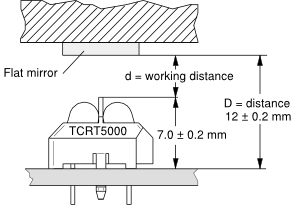
\includegraphics[width=0.5\textwidth]{reflex_test-circuit.png}%
    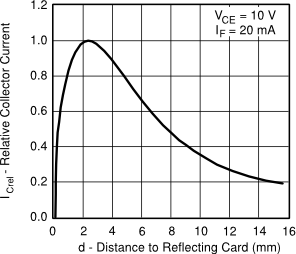
\includegraphics[width=0.5\textwidth]{reflex_working-distance.png}%
    \end{center}

    (α): \fullcite[3]{vishay09:test-circuit}

    (β): \fullcite[4]{vishay09:working-distance}
\end{figure}

Για τις ανάγκες της συσκευής, επιλέγεται λειτουργική απόσταση 2.5~cm έτσι ώστε ο
συντελεστής σύζευξης να ευνοείται όσο το δυνατόν περισσότερο.

\subsubsection{Διάστημα εναλλαγής}
Για τις ανάγκες της υλοποίησης, ο άξονας περιστροφής επικαλύπτεται, στο ύψος του
αισθήτηρα, από διαδοχικά τμήματα υψηλότερου και χαμηλότερου συντελεστή
ανάκλασης. Καθώς ο άξονας περιστρέφεται, η ένταση ρεύματος του συλλέκτη
μεταβάλλεται από τη μέγιστη μέχρι την ελάχιστη δυνατή και αντίστροφα.
Ωστόσο, σύμφωνα με το εγχειρίδιο της \textcite{vishay06}, εάν το πάχος των
τμημάτων είναι πολύ μικρό, ενδέχεται οι εναλλαγές να μην εκδηλώνονται αισθητά
στην ένταση ρεύματος του συλλέκτη.

Στο σχήμα \ref{fig:reflex:switching-distance} παρουσιάζεται η ένταση ρεύματος
του συλλέκτη για δύο διαδοχικά τμήματα.
Το σημείο εναλλαγής από τον ένα συντελεστή ανάκλασης στον επόμενο σημειώνεται
με το $Xo$ ενώ με $I_{c1}$ και $I_{c2}$, η μέγιστη ένταση ρεύματος του
συλλέκτη όταν η κοινή επιφάνεια $g$ των οπτικών πεδίων πομπού και δέκτη
καλύπτεται πλήρως από τμήμα του αντίστοιχου συντελεστή.
Προκύπτει ότι, ενώ η μετάβαση από τον ένα συντελεστή στον επόμενο συμβαίνει
ακαριαία, η ένταση ρεύματος του συλλέκτη $I_C$ έχει αρχίσει να μειώνεται σε
προγενέστερη μετατόπιση, όταν ένα πρώτο τμήμα των αρχικά διαθέσιμων ακτίνων
αποκόπηκε από το δέκτη, και συνεχίζει να μειώνεται σταδιακά έως ότου το τμήμα με
το νέο συντελεστή έχει καλύψει πλήρως την περιοχή $g$.

Επίσης, συμπαιρένεται ότι, καθώς το πάχος των τμημάτων μειώνεται ώστε η περιοχή
$g$ να είναι αδύνατο να καλυφθεί εξ ολοκλήρου από ένα μόνο τμήμα, η μέγιστη και
ελάχιστη τιμή έντασης ρεύματος που είναι δυνατό να σημειωθούν αρχίζουν να
συγκλίνουν, εφόσον, πλέον, σε κάθε μετατόπιση καταφθάνουν στο δέκτη ακτίνες από
όλο και περισσότερα τμήματα.

Το ελάχιστο πάχος τμημάτων καθορίζεται από το
\emph{διάστημα εναλλαγής}\index{διάστημα εναλλαγής} (\emph{switching distance}),
$X_d$, το οποίο ορίζεται ως το διάστημα μεταξύ δύο διαδοχικών τμημάτων
διαφορετικών συντελεστών ανάκλασης στο οποίο παρατηρείται το 90~\% $I_{C_1}$ έως
το 10~\% $I_{C2}$ \parencite{vishay06}. Η τιμή του διαστήματος εναλλαγής
εξαρτάται, από την κατασκευή του αισθητήρα καθώς και τη λειτουργική απόσταση,
ενώ όσο πιο μικρή απόσταση εναλλαγής υποστηρίζει κάποιος αισθητήρας, τόσο
υψηλότερη η διακριτική ικανότητά (resolution) του
\parencites{vishay02}{vishay06}. Για τον αισθητήρα TCRT5000, το διάστημα
εναλλαγής ανέρχεται στα 1.9~mm \parencite{vishay02}.

\begin{figure}
    \caption{Σχέση μεταβολής ρεύματος $I_C$ και συντελεστή ανάκλασης.
    \label{fig:reflex:switching-distance}}
    \begin{center}%
    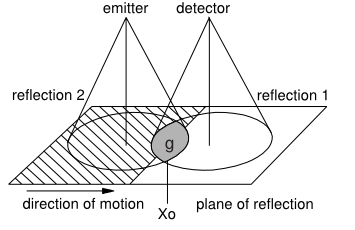
\includegraphics[width=0.4\textwidth]{reflex_switching-distance_a.png}%
    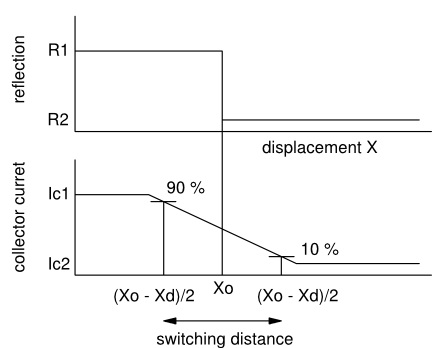
\includegraphics[width=0.5\textwidth]{reflex_switching-distance_b.png}%
    \end{center}

    \fullcite[3]{vishay06:switching-distance}
\end{figure}

\subsubsection{Θερμοκρασία}
Η αύξηση θερμοκρασίας επηρεάζει την απόδοση τόσο της διόδου εκπομπής υπερύθρων,
η οποία μειώνεται, όσο και του φωτοτρανζίστορ, η οποία αυξάνεται
\parencite{vishay06}. Ωστόσο, όπως προκύπτει από το σχήμα
\ref{fig:reflex:t-amb_ctr-rel}, για θερμοκρασίες από -10~°C έως 70~°C, το
συνολικό αποτέλεσμα επηρεάζεται ελάχιστα. Θα μπορούσε, είτε να αγνοηθεί
πλήρως είτε να συμπεριληφθεί ως σταθερή μείωση του σχετικού λόγου μεταφοράς
ρεύματος.

\begin{figure}
    \caption{Σχέση θερμοκρασίας και Λόγου μεταφοράς ρεύματος.
    \label{fig:reflex:t-amb_ctr-rel}}
    \begin{center}%
    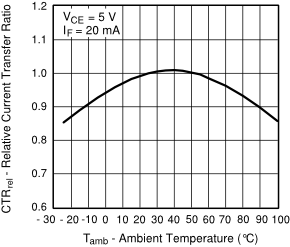
\includegraphics[width=0.5\textwidth]{reflex_t-amb_ctr-rel.png}
    \end{center}

    \fullcite[3]{vishay09:test-circuit}
\end{figure}
